\chapter{Evaluation}
\label{eval}

In diesem Kapitel soll das DXRaft evaluiert und mit ähnlichen aktuellen Systemen verglichen werden. Dazu werden in \ref{systems} zunächst einige andere Systeme vorgestellt. Dann werden in \ref{latency} und \ref{throughput} die Ergebnisse des Benchmarks mit diesen Systemen anhand der Metriken Latenz und Durchsatz erläutert. Danach wird in \ref{dxraft-latency} genauer untersucht, wie die Latenz in DXRaft zustande kommt. Zusätzlich wird in \ref{leader-election} die Performance der Systeme im Fehlerfall untersucht. Anschließend werden die Ergebnisse in \ref{summary} zusammengefasst.

\section{Andere Systeme}
\label{systems}

\subsection{Zookeeper}

Zookeeper \cite{zookeeper} ist ein Open-Source-Projekt der Apache Software Foundation. Es bietet für verteilte Systeme Möglichkeiten zur Koordinierung, Synchronisierung und einen zentralen Speicher für Konfigurationsdaten. Das System basiert auf dem Zab-Algorithmus (siehe \ref{zab}), um Konsistenz und Zuverlässigkeit zu erreichen.

Das System ist auf einer einfachen Client-Server-Struktur aufgebaut. Die Zookeeper-Server nehmen am Konsensus-Algorithmus teil und bearbeiten die Anfragen von Clients. Es ist es auch möglich, Server im \textit{Observer}-Modus zu starten. Dann nimmt der Server nicht am Konsensus-Algorithmus, sondern bekommt nur die Entscheidungen mitgeteilt. Dadurch kann die Last des Systems auf mehr Server verteilt werden, ohne dass die Performance von Write-Anfragen darunter leidet. Das ist vor allem dann von Vorteil, wenn sehr viele Clients auf Zookeeper zugreifen sollen. \\
Der Client wird von Anwendungen als Bibliothek genutzt und baut eine Verbindung zu den Servern auf. Zookeeper ist in Java implementiert und Client-Bibliotheken existieren für Java und C. \\
Zookeeper stellt hauptsächlich einen hierarchischen Key-Value-Store zur Verfügung, der einem Dateisystem ähnelt. Die Knoten in diesem Namensraum werden \textit{znodes} genannt. Jeder \textit{znode} hat einen Pfad, der die Beziehung zu den anderen Knoten im Namensraum festlegt. Außerdem kann jeder \textit{znode} Daten speichern. Zusätzlich dazu werden Metadaten über den Knoten gespeichert wie Versionsnummern und Zeitstempel. Mit einer Access Control List kann für jeden \textit{znode} festgelegt werden, wer welche Operation auf diesem Knoten durchführen darf. Clients öffnen beim Verbindungsaufbau eine Session. \textit{znodes} können mit einer Session verknüpft werden und dann automatisch gelöscht werden, wenn diese Session ausläuft. Beim Lesen von Daten kann der Client eine \textit{Watch} setzen. Dann wird er einmalig benachrichtigt, sobald die gelesenen Daten geändert wurden.\\
Beim Lesen von Daten ist wichtig zu beachten, dass Zookeeper nicht garantiert, dass die neuesten Daten gelesen werden. Wenn also Client A den Wert von \textit{znode} /a von 0 auf 1 ändert, Client B benachrichtigt und Client B dann /a liest, kann es sein, dass Client B den Wert 0 liest. Das liegt daran, dass das Lesen von Daten nicht über den Zab-Algorithmus läuft, sondern von den Zookeeper-Server direkt aus den lokalen Daten gelesen wird. Dadurch können Leseanfragen deutlich schneller bearbeitet werden. Da die Clients sich mit unterschiedlichen Servern verbinden können, ist nicht garantiert, dass zwei Client stets die gleiche Sicht auf die Daten haben. Es existiert jedoch ein Befehl \textit{sync()}, den Clients aufrufen können. Dadurch synchronisiert sich der verbundene Server mit dem restlichen Cluster und es können die neuesten Daten gelesen werden. \\
Da Zookeeper selbst nur einen Key-Value-Store anbietet, gibt es mit Apache Curator \cite{curator} eine zusätzliche Client-Bibliothek, die abstraktere Datenstrukturen und Werkzeuge bietet und die Verwendung von Zookeeper vereinfacht. \\
In den Benchmarks wird Zookeeper in der Version 3.4.13 und der Java-Client genutzt.

\subsection{Consul}

Consul \cite{consul} ist ein Open-Source-Projekt von Hashicorp. Ähnlich wie Zookeeper bietet es einen zuverlässigen und konsistenten Key-Value-Store für verteilte Systeme. Zusätzlich werden weitere Features wie Service-Discovery (Dienste registrieren sich zentral in Consul und andere Dienste können diese dort finden) und Health-Checking (Clients können den Status von Diensten und Servern ermitteln). Der Key-Value-Store basiert auf dem Raft-Algorithmus (siehe \ref{raft}). \\
Ein Consul Prozess heißt \textit{Agent} und kann im Client- oder Server-Modus gestartet werden. Im Server-Modus nimmt der \textit{Agent} am Konsensus-Algorithmus teil. Im Client-Modus verbindet sich der \textit{Agent} für die meisten Operationen mit einem \textit{Agent} der im Server-Modus läuft, und leitet die Anfragen weiter. \\
Anwendungen können über eine HTTP-REST-Schnittstelle, die jeder \textit{Agent} bereitstellt, auf die Consul-Dienste zugreifen. Für die Service-Discovery kann zusätzlich eine DNS-Schnittstelle genutzt werden.\\
Der Zugriff kann wie bei Zookeeper ebenfalls über eine Access-Control-List geschützt werden. Der Key-Value-Store ist jedoch nicht hierarchisch aufgebaut. \\
Für die Leseanfragen gibt es drei verschiedene Konsistenzmodi, die für jede Anfrage festgelegt werden können:

\begin{itemize}
	\item \textbf{default}: Stark konsistent in den meisten Fällen. Bei einem Leaderwechsel können jedoch alte Werte gelesen werden, um die Anfragen schneller zu beantworten.
	\item \textbf{consistent}: In allen Fällen stark konsistent. Der Leader fragt das Cluster dabei, ob er noch Leader ist, sodass keine inkonsistenten Daten gelesen werden können. Dafür dauert das Lesen länger.
	\item \textbf{stale}: Jeder Consul-Server kann die Leseanfrage beantworten. Dadurch können beliebig alte Werte gelesen werden. Dafür werden die Leseanfragen schneller bearbeitet und auch ein Cluster ohne Leader kann Leseanfragen beantworten.
\end{itemize}

Im Benchmark wird Consul in Version 1.4.3 und ein Java-Client \cite{consul-client} genutzt, der auf die HTTP-Schnittstelle zugreift.

\subsection{etcd}

etcd \cite{etcd} ist ein zuverlässiger Key-Value-Store für verteilte System von CoreOS. Das System ist in Go implementiert und basiert ebenfalls auf dem Raft-Algorithmus. Es wird in der Industrie verbreitet eingesetzt, z.B. im Container-Orchestrierungs-System Kubernetes \cite{kubernetes}.

Wie die anderen Systeme nutzt auch etcd eine Client-Server-Struktur, bei der die Server den Konsensus-Algorithmus durchführen. Die Clients kommunizieren mit den Servern über eine HTTP-REST-Schnittstelle oder über gRPC, ein plattformübergreifendes Remote-Procedure-Call-Protokoll. Eine Besonderheit des Key-Value-Stores ist, dass die History der Keys gespeichert bleibt und alte Versionen weiterhin gelesen werden können. Außerdem können mehrere Anfragen in Transaktionen zusammengeschlossen werden und Clients können Keys überwachen, indem sie Watches darauf setzen und dann mitgeteilt bekommen, wenn sich die Daten ändern.

Auch etcd bietet unterschiedliche Konsistenzmodi für Leseanfragen. Standardmäßig sind die Leseanfragen linearisierbar, um die Leseanfragen schneller zu bearbeiten, können per Parameter auch alte Daten erlaubt werden. Es gibt es viele verschiedene Client\hyp{}Implementierungen in unterschiedlichen Sprachen. Im Benchmark in dieser Arbeit wird etcd in der Version 3.3.12 und der Java-Client jetcd \cite{jetcd} verwendet.

\section{Latenz}
\label{latency}

\begin{figure}[t]
	\centering
	\begin{subfigure}[t]{0.45\textwidth}
		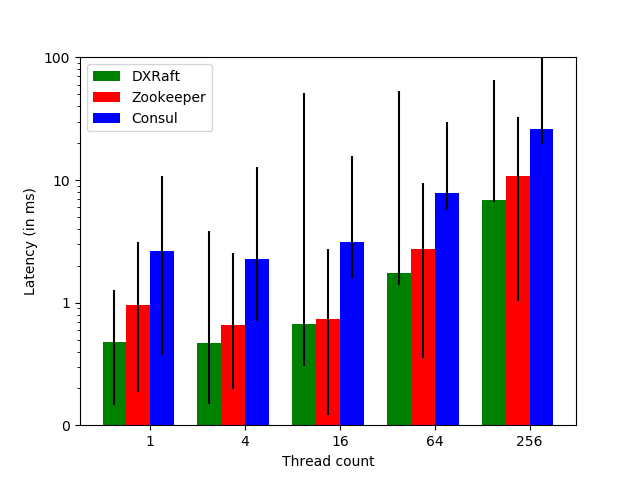
\includegraphics[width=\textwidth]{img/latency.png}
		\caption{100\% Writes.}
	\end{subfigure}
	\begin{subfigure}[t]{0.45\textwidth}
		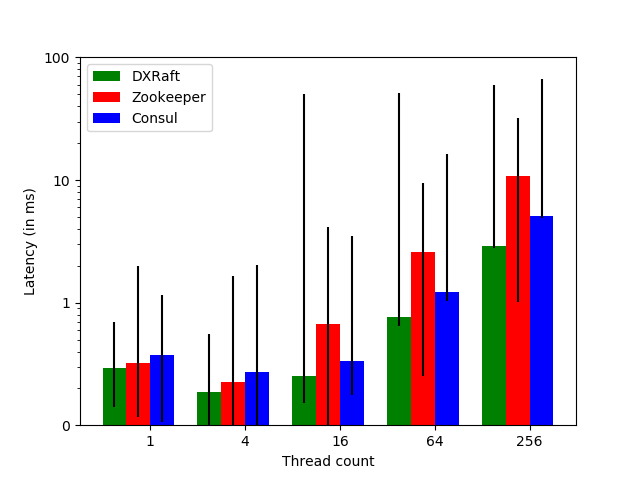
\includegraphics[width=\textwidth]{img/latency2.png}
		\caption{25\% Writes, 75\% Reads.}
	\end{subfigure}
	\caption{Latenzen der Systeme. Der Benchmark wurde mit einem Client und drei Server durchgeführt.}
	\label{fig:latency}
\end{figure}

Um die Performance der Systeme zu messen, ist zunächst die Latenz wichtig, also die Zeitspanne vom Senden einer Anfrage bis zum Erhalt der Anfrage. Die Abbildung \ref{fig:latency} zeigt die Latenz der verschiedenen Systeme bei zunehmender Anzahl an Client-Threads. Die Client-Threads wurden auf einem Client ausgeführt und sendeten die Anfragen blockierend an die Systeme. Jeder Client-Thread sendete also nur eine Anfrage gleichzeitig. Die Systeme wurden auf jeweils aus drei Servern ausgeführt, die am Konsensus-Algorithmus teilnahmen. Jeder Server bestand aus einem Intel Xeon Prozessor mit 4 Cores und 32 GB RAM. Die farbigen Balken zeigen die durchschnittliche Latenz, während die schwarzen Striche den Bereich des 99,9ten Perzentils zeigen. Es wurden zwei Workloads getestet: Ein Workload mit 100 \% Writes zeigt die Performance der Konsensus-Implementierung, da dabei alle Anfragen von allen Servern in der gleichen Reihenfolge bearbeitet werden müssen. Ein Workload mit nur 25\% Writes und 75\% Reads entspricht mehr einem realen Workload. Da Zookeeper keine linearisierbaren Leseanfragen anbietet, wurden die Leseanfragen mit abgeschwächter Konsistenz ausgeführt: Bei DXRaft und etcd wird der ebenfalls keine Linearisierbarkeit gefordert und bei Consul wird der Konsistenzmodus \textit{stale} verwendet. Bei linearisierbaren Lesanfragen würden die Ergebnisse vermutlich stark den Ergebnissen des Workloads mit aussschließlich Schreibanfragen ähneln, da diese dann ebenfalls den Konsensus-Algorithmus durchlaufen müssen.

Insgesamt ist die durchschnittliche Latenz bei DXRaft am geringsten. Die anderen Systeme scheinen also etwas mehr Arbeit pro Anfrage zu verrichten. Möglicherweise könnte dies an fehlenden Features in DXRaft liegen, wie z.B. eine Log-Kompaktierung, die nebenläufige Arbeit erfordert. Dennoch scheint DXRaft im Vergleich mit den anderen Systemen im Durschnitt gute Latenzen zu haben. Etwas schlechter ist die durchschnittliche Latenz bei Zookeeper und etcd, die etwa gleichauf liegen. Bei Consul ist diese im Vergleich zu den anderen Systemen deutlich höher.

Im 99,9ten Perzentil nimmt bei DXRaft die maximale Latenz im Vergleich zum Durchschnitt mit steigender Anzahl an Anfragen deutlich zu. Dies lässt sich bei den anderen Systemen nicht beobachten. Die Latenzen von DXRaft sind also deutlich weniger stabil als die Latenzen bei den anderen Systemen. Hier könnte DXRaft eventuell durch mehr Parallelität und bessere Messaging-Implementierung stabiler werden, z.B. durch das gleichzeitige Versenden mehrerer Append-Entries-Request des Leaders an die Follower. Auch das Minimum im 99,9ten Perzentil nähert sich bei DXRaft mit steigender Anzahl an Anfragen immer mehr dem Durchschnitt. Dies lässt sich bei Consul ebenso beobachten. Bei Zookeeper ist dagegen ist auch das Minimum im Vergleich zum Durchschnitt sehr stabil.

Bei bis zu 16 Threads steigen die Latenzen nicht stark an. Bei Consul, Zookeeper und etcd nehmen die Latenzen sogar zunächst im Vergleich zu einem einzelnen Thread ab. Dies könnte durch eine Bearbeitung in Batches und durch höhere Parallelität hervorgerufen werden. Bei DXRaft ist jedoch keine Abnahme der Latenz von Schreibanfragen zu erkennen. Möglicherweise könnte hier durch mehr Parallelität ebenfalls die Latenz verringert werden, z.B. durch mehrere Message-Handler-Threads.

Bei dem Workload mit 75\% Reads sind die Latenzen insgesamt erwartungsgemäß niedriger. Ansonsten ändert sich wenig: DXRaft hat weiterhin die geringsten durchschnittlichen Latenzen, jedoch sind diese weniger stabil. Ein Unterschied ist jedoch, dass Consul bei diesem Workload ab 16 Threads eine deutlich bessere durchschnittliche Latenz hat im Vergleich zu Zookeeper und etcd. Die Leseanfragen im Konsistenzmodus \textit{stale} scheinen bei Consul also sehr gut optimiert zu sein, während die Schreibanfragen eher weniger gut optimiert sind.

\section{Durchsatz}
\label{throughput}

Neben der Latenz ist auch der Durchsatz der Systeme wichtig, also die Anzahl an verarbeiteten Anfragen pro Zeiteinheit. Abbildung \ref{fig:throughput} zeigt den Durchsatz der Systeme beim in \ref{latency} beschriebenem Benchmark. Dies entspricht in etwa den Ergebnissen des Vergleichs der Latenzen: DXRaft hat den höchsten Durchsatz, bei Schreibanfragen hat Zookeeper den zweithöchsten Durchsatz und mit Leseanfragen hat Consul den zweithöchsten Durchsatz.

Interessant ist hierbei, dass der maximale Durchsatz bei Zookeeper bereits bei 16 Threads erreicht zu sein scheint, da er bei mehr Threads nicht mehr steigt. Bei DXRaft steigt der Durchsatz dagegen noch bis 64 Threads. Beim Workload mit Leseanfragen steigt der Durchsatz sogar bis 256 Threads. Dies könnte bei Leseanfragen durch eine bessere Verteilung der Anfragen auf die Server zustande kommen. Da die Leseanfragen nicht linearisierbar sein müssen, können diese von jedem Server im Cluster bearbeitet werden. In DXRaft wird deswegen im Client ein zufälliger Server gewählt, an den die Anfrage geschickt wird. Da der Durchsatz bei Consul, Zookeeper und etcd mit Leseanfragen ab 16 Threads nicht mehr steigt, scheinen die Anfragen nicht gut auf alle Server verteilt werden. Dies kann bei Consul und etcd auch an den Client-Implementierungen liegen, die nicht direkt von den Teams selbst gepflegt werden.

\begin{figure}[t]
	\centering
	\begin{subfigure}[t]{0.45\textwidth}
		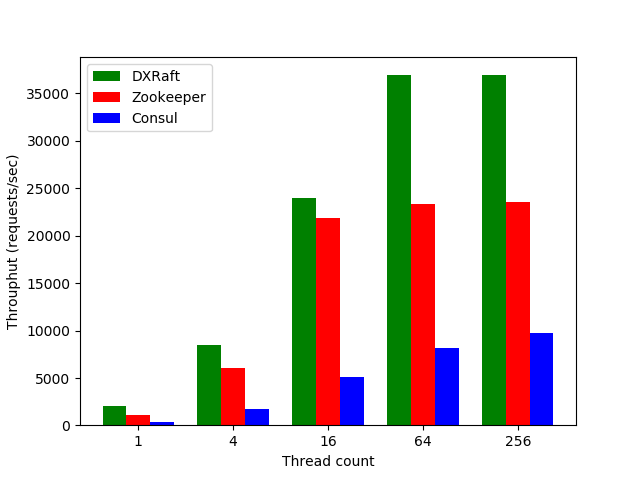
\includegraphics[width=\textwidth]{img/throughput.png}
		\caption{100\% Writes.}
	\end{subfigure}
	\begin{subfigure}[t]{0.45\textwidth}
		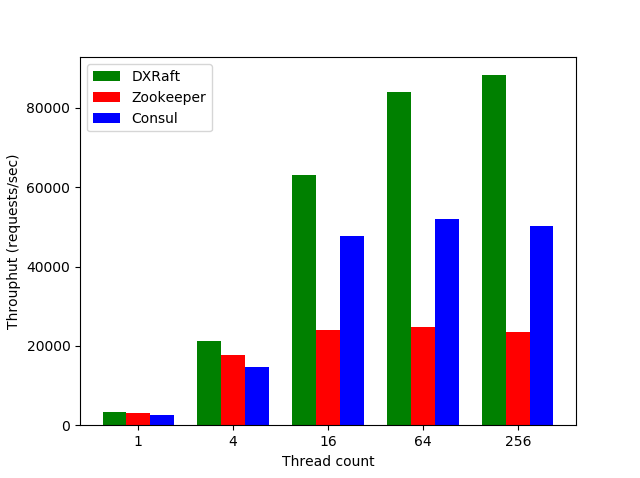
\includegraphics[width=\textwidth]{img/throughput2.png}
		\caption{25\% Writes, 75\% Reads.}
	\end{subfigure}
	\caption{Durchsatz der Systeme. Der Benchmark wurde mit einem Client und drei Server durchgeführt.}
	\label{fig:throughput}
\end{figure}


\section{Latenz in DXRaft}
\label{dxraft-latency}

\begin{figure}[t]
	\centering
	\begin{subfigure}[t]{1\textwidth}
		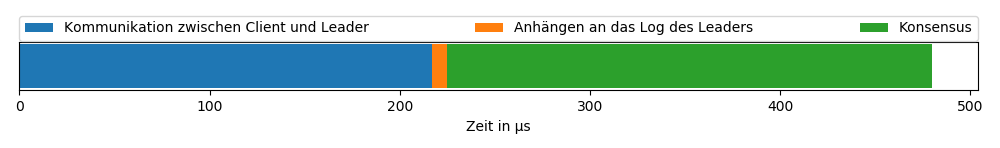
\includegraphics[width=\textwidth]{img/request_avg_timing.png}
		\caption{Durchschnittliche Anfrage.}
		\label{fig:request-avg}
	\end{subfigure}
	\begin{subfigure}[t]{1\textwidth}
		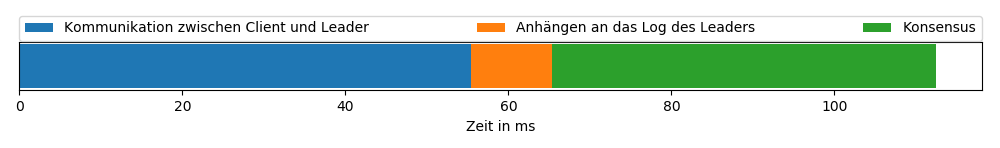
\includegraphics[width=\textwidth]{img/request_max_timing.png}
		\caption{Maximale Zeiten.}
		\label{fig:request-max}
	\end{subfigure}
	\begin{subfigure}[t]{1\textwidth}
		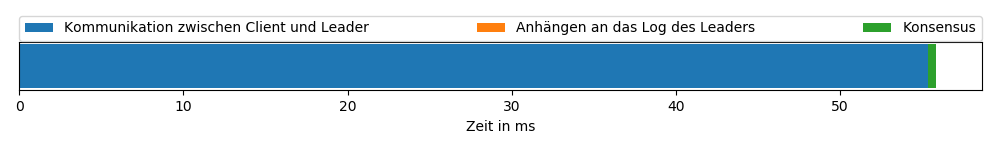
\includegraphics[width=\textwidth]{img/request_longest_timing.png}
		\caption{Längste Anfrage.}
		\label{fig:request-longest}
	\end{subfigure}
	\caption{Aufteilung der Latenz in DXRaft.}
	\label{fig:latency-analysis}
\end{figure}

Um das Optimierungspotenzial von DXRaft zu bestimmen, kann die Aufteilung der Latenz der Anfragen ermittelt werden. Dabei kann die Bearbeitung einer (Schreib-)Anfrage in folgende Aktionen aufgeteilt:
\begin{itemize}
	\item \textbf{Kommunikation zwischen Client und Leader}: Zeit, den die Kommunikation von Client und Leader benötigt, also Senden der Anfrage, erhalten der Anfrage, senden der Antwort und erhalten der Antwort. Diese wird ermittelt, indem von der beim Client ermittelten gesamten Laufzeit der Anfrage die Zeit für die Leader-Aktionen abgezogen wird.
	\item \textbf{Anhängen an das Log des Leaders}: Um eine Schreibanfrage auszuführen, muss der Leader einen Log-Eintrag erstellen und diesen an sein Log anhängen. Da das Log auf Festplatte persistiert werden muss, schließt dies einen Schreibzugriff auf die Festplatte mit ein und ist deswegen interessant.
	\item \textbf{Konsensus}: Zeit, um den Log-Eintrag auf eine Mehrheit der Follower zu replizieren. Dies schließt also die Kommunikation mit einer Mehrheit der Follower und die Verarbeitung des Eintrags bei den Followern ein. Dabei muss der Log-Eintrag auch vom Follower an sein Log angehängt werden, sodass dieser ebenfalls auf die Festplatte schreiben muss.
\end{itemize}

Interessant sind vor allem die Schreibanfragen, da diese durch den Konsensus-Algorithmus laufen müssen und dadurch länger benötigen als Leseanfragen. Abbildung \ref{fig:latency-analysis} visualisiert, welche Aktionen wie viel Zeit benötigen. Die Daten wurden mit einem Cluster aus drei DXRaft-Servern und einem Client mit vier Threads ermittelt. \\

In \ref{fig:request-avg} ist die durchschnittliche Dauer der beschriebenen Aktionen dargestellt. Im Durchschnitt lässt sich vor allem erkennen, dass die Zeit für das Anhängen an das Log sehr kurz ist und somit keinen Flaschenhals darstellt, obwohl dabei auf die Festplatte geschrieben werden muss. Die größte Zeit geht offensichtlich bei der Kommunikation verloren, etwa in gleichem Maße zwischen Client und Leader und zwischen Leader und Follower. Wenn die durchschnittliche Latenz noch verbessert werden sollte, könnte man also bei beiden Kommunikationen ansetzen. \\

In \ref{fig:request-max} ist die maximale Dauer der Aktionen dargestellt. Dabei ist festzustellen, dass auch die maximale Dauer der Kommunikation zwischen Client und Leader und zwischen Leader und Follower ähnlich groß ist. Insgesamt ist das Maximum mit etwa 40-50 ms bei beiden Kommunikationsaktionen sehr groß, insbesondere im Vergleich zum Durchschnitt. Es sollte mit den beschriebenen Optimierungsmöglichkeiten, z.B. mehr Parallelisierung bei der Verarbeitung von Nachrichten, möglich sein, das Maximum zu senken. Möglicherweise könnte auch der Garbage Collector dafür sorgen, dass die Nachrichtenverarbeitung unterschiedlich lange benötigt. Hier könnte mit anderen Garbage Collectoren experimentiert werden, die möglichst wenige Pausen der Anwendung verursachen.

Interessant ist auch die Verteilung bei der Anfrage, die die längste Zeit benötigt hat. Diese ist in \ref{fig:request-longest} zu sehen. Dabei ist auffällig, dass bei der längsten Anfrage die Zeit fast ausschließlich bei der Kommunikation zwischen Client und Leader verloren gegangen ist. Um das Maximum zu senken, sollte also zunächst diese Kommunikation betrachtet werden. Hier könnte möglicherweise der Session-Mechanismus Auslöser sein, da das Leeren der Session eine zusätzliche Anfrage benötigt (siehe \ref{sessions} für eine Beschreibung des Session-Mechanismus). Die Zeit für diese Anfrage fällt ebenfalls in die Kommunikation zwischen Client und Leader, da die Zeiten nur für die eigentliche Anfrage gemessen wurden.

\section{Leader Election}
\label{leader-election}

Für die Bewertung des Systems ist nicht nur die Performance unter optimalen Bedingungen wichtig, sondern auch die Toleranz von Ausfällen. Dies ist gerade die Motivation für die Entwicklung des Systems. Leider ist es schwierig, eine Netzwerkpartitionierung zu simulieren. Eine Ausfall eines oder mehrerer Server lässt sich dagegen einfacher hervorrufen. Der Ausfall eines Followers ist weniger interessant als der eines Leaders, da sich der Ablauf der Anfrageverarbeitung beim Ausfall eines Followers kaum ändert. Bei dem Ausfall des Leaders muss dagegen das Cluster den Ausfall erkennen, einen neuen Leader bestimmen und die Anfragen müssen zum neuen Leader geleitet werden. \\
Abbildung \ref{fig:leader-crash} zeigt die Entwicklung der durchschnittlichen und maximalen Latenz mit der Zeit. Die Daten wurden wieder mit dem gleichen Benchmark wie zuvor ermittelt, mit drei Servern und einem Client mit vier Threads. Dabei wurde jeweils während der Laufzeit der Leader-Prozess zum Absturz gebracht. Dies geschah etwa zwischen Sekunde 20 und 30. \\
Die Clients von Zookeeper, Consul und etcd werfen bei einem Verbindungsabbruch zum Leader eine Exception, die die Anwendung davon benachrichtigt. Diese wurden ignoriert und die Anfragen wurden sofort erneut gesendet, um möglichst schnell eine Antwort zu erhalten. Das finden des neuen Leaders wird jedoch von den Clients automatisch übernommen. Bei DXRaft wird das erneute Senden der Anfragen bereits automatisch vom Client übernommen, solange eine bestimmte Zeit nicht überschritten wird. \\
Auf der Abbildung ist jeweils der Zeitpunkt des Leader-Ausfalls klar zu erkennen. Da der Durchschnitt und das Maximum über den Zeitraum von einer Sekunde bestimmt wurde, ist bei Zookeeper und Consul eine Lücke im Graphen, die aussagt, dass in dieser Sekunde keine Anfrage verarbeitet wurde. Es ist festzustellen, dass es nach dem Ausfall des Leaders bei DXRaft nur etwa eine Sekunde dauert, bis Anfragen wieder verarbeitet werden können. Auch bei etcd scheint der Ausfall sehr schnell erkannt zu werden und durch die Wahl eines neuen Leaders behoben zu werden. Bei Zookeeper dauert dies etwas länger, etwa 2-3 Sekunden. Bei Consul werden sogar über 10 Sekunden keine Anfragen beantwortet. Diese Ausfallerkennung oder die Leader Election scheint bei Consul also sehr viel Zeit zu benötigen, obwohl Consul ebenso wie DXRaft und etcd Raft als Algorithmus nutzt. DXRaft scheint den Ausfall des Leaders dagegen, auch im Vergleich mit den anderen Systemen, schnell kompensieren zu können. \\
Interessant ist außerdem, dass die durchschnittliche Latenz bei DXRaft nach dem Ausfall eines Servers zunimmt. Bei Zookeeper und Consul bleibt diese etwa gleich, während sie bei etcd sogar abnimmt. Zu erwarten ist eigentlich, dass die Latenz etwa gleich bleibt, da der Cluster aus drei Servern bestand und der Leader jede Anfrage sowohl vor als auch nach dem Ausfall auf mindestens einen anderen Server replizieren muss, bevor er die Ausführung der Anfrage bestätigt. \\
Auffällig ist, dass die maximale Latenz bei DXRaft sehr regelmäßig bei etwa 50 ms liegt, was auch im Vergleich zu den anderen Systemen sehr hoch ist. Normalerweise ist die maximale Latenz deutlich unregelmäßiger, wie bei den anderen Systemen zu sehen. Dies sollte genauer untersucht werden, falls die Performance von DXRaft verbessert werden soll.


\begin{figure}[t]
	\centering
	\begin{subfigure}[t]{0.45\textwidth}
		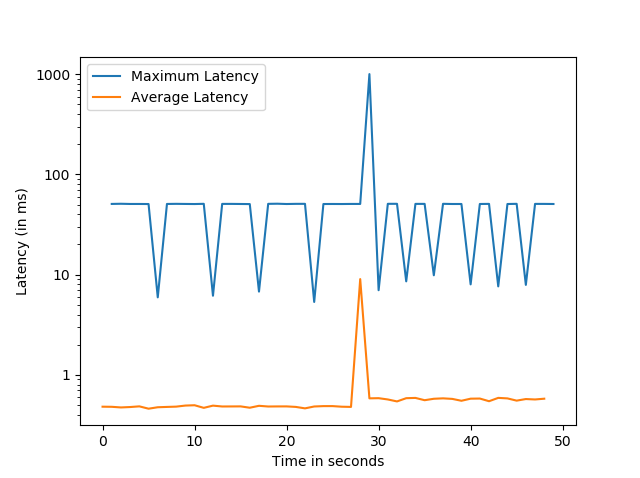
\includegraphics[width=\textwidth]{img/leader_crash_dxraft.png}
		\caption{DXRaft.}
	\end{subfigure}
	\begin{subfigure}[t]{0.45\textwidth}
		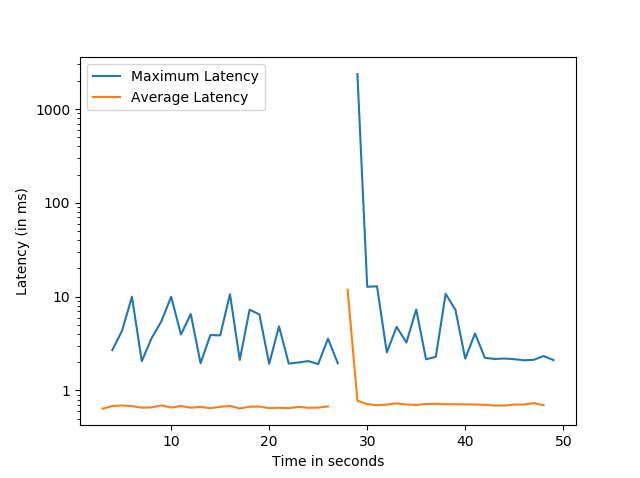
\includegraphics[width=\textwidth]{img/leader_crash_zk.png}
		\caption{Zookeeper.}
	\end{subfigure}
	\begin{subfigure}[t]{0.45\textwidth}
		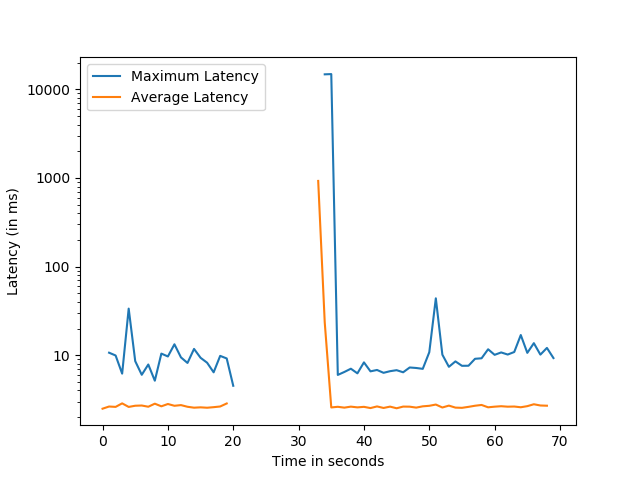
\includegraphics[width=\textwidth]{img/leader_crash_consul.png}
		\caption{Consul.}
	\end{subfigure}
	\begin{subfigure}[t]{0.45\textwidth}
		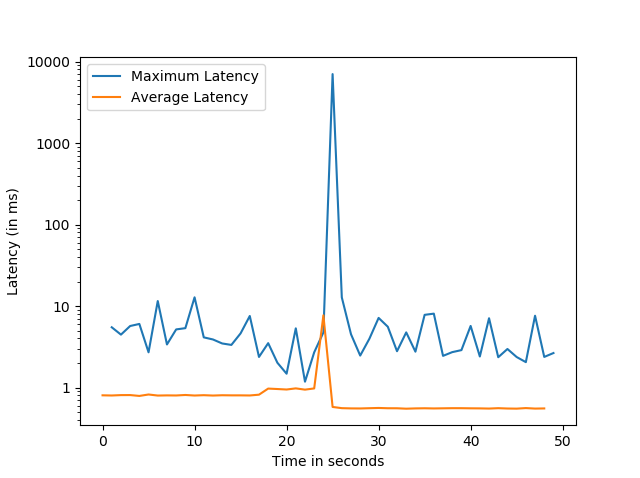
\includegraphics[width=\textwidth]{img/leader_crash_etcd.png}
		\caption{etcd.}
	\end{subfigure}
	\caption{Latenz bei einem Leader-Crash.}
	\label{fig:leader-crash}
\end{figure}

\section{Zusammenfassung}
\label{summary}

Zusammenfassend kann man sagen, dass DXRaft sowohl bei der Latenz als auch beim Durchsatz mit aktuellen, in der Industrie eingesetzten ähnlichen Systemen mithalten und teilweise sogar übertreffen kann. Die Latenzen sind deutlich weniger stabil im Vergleich zu den anderen getesteten Systemen. Der Engpass dabei scheint vor allem die Kommunikation zu sein, sowohl zwischen Client und Server als auch zwischen den Servern. Bei einem Ausfall des Leaders kann schnell ein neuer Leader gewählt werden, sodass schnell wieder Anfragen bearbeitet werden können. 

Die Diskrepanz der gemessenen Werte von DXRaft zu den anderen getesteten Systemen könnte an fehlenden Features wie z.B. die Log-Kompaktierung, liegen. Möglicherweise implementieren die anderen Systeme auch noch weitere Sicherheitsfeatures, z.B. die Überprüfung der von der Festplatte gelesenen Daten auf Fehler. Bei der Entwicklung solcher Systeme wird die Sicherheit vermutlich höher priorisiert als die Performance, da die Systeme im Produktiveinsatz meist wenige wichtige Daten speichern und für die Speicherung sehr vieler Daten durch die Konsistenzgarantien, die Performance kosten, ohnehin nicht geeignet sind.


